\documentclass[11pt]{article}
\usepackage{amsmath}
\usepackage{fancyhdr}
\usepackage[hidelinks]{hyperref}
\usepackage{graphicx}
\newcommand{\compactlist}{\setlength{\itemsep}{0pt} \setlength{\parskip}{0pt} \setlength{\leftskip}{-1em}}
\usepackage[margin=1in]{geometry}

\lhead{MATH 4363/5373}
\rhead{Oct. 30, 2019}
\chead[RE]{Orthogonal functions}
\cfoot{}
%\rfoot[RO]{Code for figure and report is available in the class folder.}

\pagestyle{fancy}
\begin{document}
%%%%%%%%%%%%%%%%%%%%%%%%%%
%%%%%%%%%%%%%%%%%%%%%%%%%%
\section{Orthogonal polynomials}
\subsection{Legendre polynomials}
The standard monomials for function approximation, shown as the familiar unlabeled gray curves in Figure~\ref{fig::leg}, are \(\phi_i(x) = x^i\) for \(i=0, 1, \dots, n\).  These lack the property of orthogonality that is achieved by the Legendre polynomials, also shown Figure~\ref{fig::leg}, but in black and labeled.  The first few Legendre polynomials are


\begin{figure}[h!]\centering

\begin{minipage}[c]{0.48\textwidth}
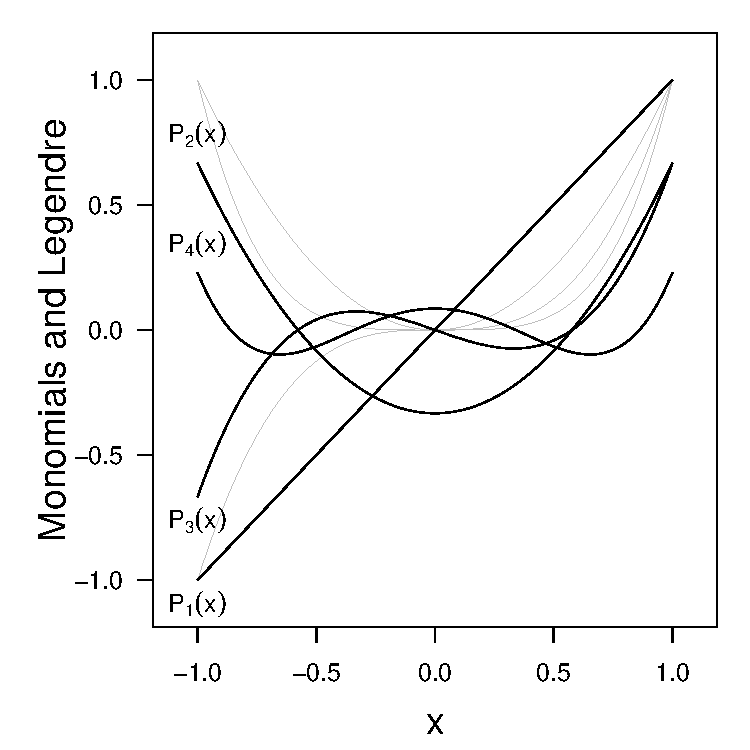
\includegraphics[width=\textwidth]{legendre_funs.pdf}

\end{minipage}
\begin{minipage}[c]{0.48\textwidth}
\begin{align*}
P_0(x) & = 1\\
P_1(x) & = x\\
P_2(x) & = x^2-\dfrac{1}{3}\\
P_3(x) & = x^3-\dfrac{3}{5}x\\
 & \dots\\
P_n(x) & = (x-B_k)P_{n-1}(x)-C_kP_{x-2}(x)
\end{align*}

where
\begin{align*}
B_k & = \dfrac{\int_{-1}^1 x \cdot 1 \cdot [P_{k-1}(x)]^2\,dx}{\int_{-1}^1 1 \cdot [P_{k-1}(x)]^2\,dx}\\
C_k & = \dfrac{\int_{-1}^1 x \cdot 1 \cdot [P_{k-1}(x) P_{k-2}(x)]\,dx}{\int_{-1}^1 1 \cdot [P_{k-2}(x)]^2\,dx}
\end{align*}

\caption{In gray the intuitive monomials \(\phi_i(x) = x^i\) with the Legendre polynomials \(P_i(x)\) in black.}\label{fig::leg}

\end{minipage}
\end{figure}

%%%%%%%%%%%%%%%%%%%%%%%%%%
%%%%%%%%%%%%%%%%%%%%%%%%%%
\subsection{Chebyshev polynomials}
The standard monomials for function approximation, shown as the familiar unlabeled gray curves in Figure~\ref{fig::cheb}, are \(\phi_i(x) = x^i\) for \(i=0, 1, \dots, n\).  These lack the property of orthogonality that is achieved by the Chebyshev polynomials, also shown Figure~\ref{fig::cheb}, but in black and labeled. The first few Chebyshev polynomials are
%
\begin{figure}[h!]\centering

\begin{minipage}[c]{0.48\textwidth}
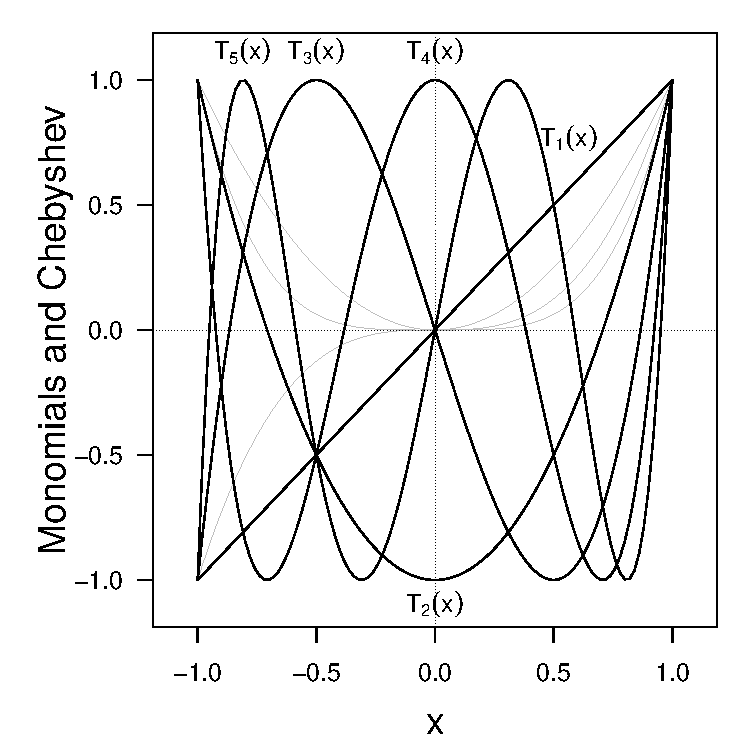
\includegraphics[width=\textwidth]{cheb_funs.pdf}

\end{minipage}
\begin{minipage}[c]{0.48\textwidth}
\begin{align*}
T_0(x) & = 1\\
T_1(x) & = x\\
T_2(x) & = 2x^2-1\\
T_3(x) & = 4x^3-3x\\
 & \dots\\
T_n(x) & = 2xT_{n-1}(x) - T_{n-2}(x)
\end{align*}

\caption{In gray the intuitive monomials \(\phi_i(x) = x^i\) with the Chebyshev polynomials \(T_i(x)\) in black.}\label{fig::cheb}

\end{minipage}
\end{figure}

Since the alternate definition of the Chebyshev polynomials is \(T_n(x) = \cos(n\arccos(x))\) for \(n\geq0\), it should seem reasonable that these functions are bounded in magnitude by one, as illustrated in Figure~\ref{fig::cheb}.  The monic Chebyshev polynomials (not illustrated, but handy for Chebyshev economization of power series), with leading coefficient \(1\), are defined by \[\tilde T_n(x) = \dfrac{1}{2^{n-1}}T_n(x)\] For these polynomials the extrema, which occur \textit{at} the same points, are those of \(T_n(x)\) but reduced in value by a factor of \(\dfrac{1}{2^{n-1}}\), that is, the extrema are, for \(k=0, 1, \dots, n\) \[\tilde T'_n(\bar x_k) = \dfrac{(-1)^k}{2^{n-1}}\]


%%%%%%%%%%%%%%%%%%%%%%%%%%
%%%%%%%%%%%%%%%%%%%%%%%%%%
\subsubsection{Chebyshev points and Lagrange nodes}
By a theorem, we have that the optimal choice of nodes for polynomial approximation by a degree \(n\) polynomial is given by the zeros of of the \((n+1)^\text{st}\) Chebyshev polynomial \(T_{n+1}(x)\).  For example, as given in Figure~\ref{fig::cheb_pts}, we take the approximation of \(f(x) = e^x\) on \([0, 1]\) with three points.  We expect to to take, \(\tilde x_0 = 0\), \(\tilde x_1 = 0.5\), and \(\tilde x_2 = 1.0\), but achieve better performance with Chebyshev nodes \(\bar x_i\).  The nodes for interpolation are given by the zeros of the Chebyshev polynomial \(T_3(x)\), which in turn are given by \(\bar x_k = \cos\left(\dfrac{2k-1}{2n}\pi\right)\) for \(k=1, 2, 3\).
\begin{align*}
\bar x_1 &= \cos\left(\dfrac{2(1)-1}{2(3)}\cdot\pi\right) = \cos\left(\dfrac{1\cdot\pi}{6}\right)= \dfrac{\sqrt{3}}{2} \approx 0.866\\
\bar x_2 &= \cos\left(\dfrac{2(2)-1}{2(3)}\cdot\pi\right) = \cos\left(\dfrac{3\cdot\pi}{6}\right)= 0\\
\bar x_3 &= \cos\left(\dfrac{2(3)-1}{2(3)}\cdot\pi\right) = \cos\left(\dfrac{5\cdot\pi}{6}\right)= -\dfrac{\sqrt{3}}{2} \approx -0.866 
\end{align*}

From \(\tilde x_i \in [a,b]\) we can compute \(\bar x_i \in [-1, 1]\) by \[x_i = \dfrac{2\tilde x_i - a - b}{b-a}\] and in the reverse we can use \[\tilde x_i = \dfrac{1}{2}\left((b-a)\bar x_i + a + b\right)\] As an example,
\begin{center}
\begin{tabular}{cll}
\(i\) & \(\phantom{-}\bar x_i\) & \(\tilde x_i\)\\
\hline \hline
& & \\[-10pt]
1 & \(\phantom{-}0.866\) & 0.933\\  
2 & \(\phantom{-}0.0\) & 0.500 \\
3 & \(-0.866\) & 0.067
\end{tabular}
\end{center}

The n\"aively chosen nodes  that include the endpoints (red) are illustrated in the left-hand panel of Figure~\ref{fig::cheb_pts}, and as shown give a reasonable approximate.  Yet, the approximation is improved by use of the Chebyshev points (blue).  
%
\begin{figure}[h!]\centering
\begin{minipage}{0.48\textwidth}
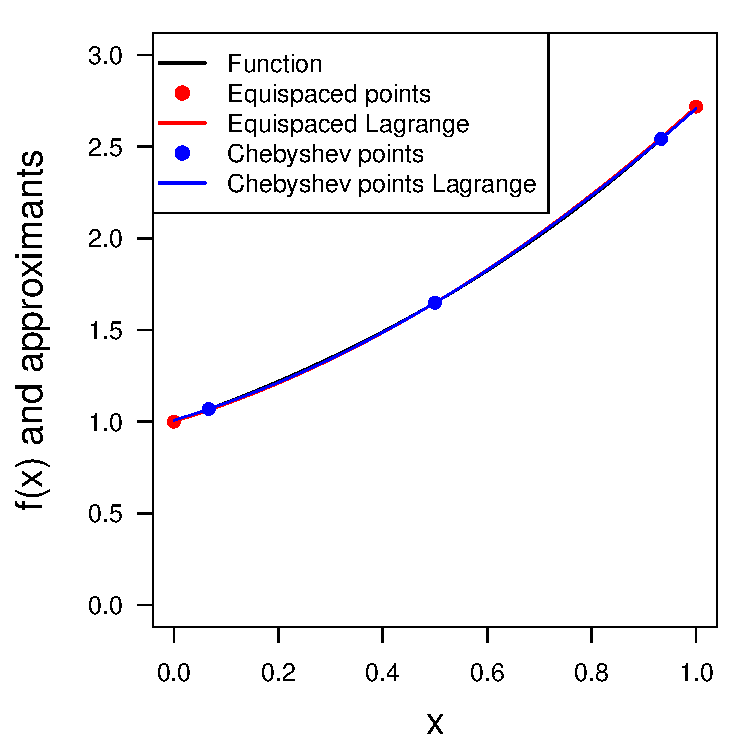
\includegraphics[width=\textwidth]{cheb_pts_lagr.pdf}

\end{minipage}
\begin{minipage}{0.48\textwidth}

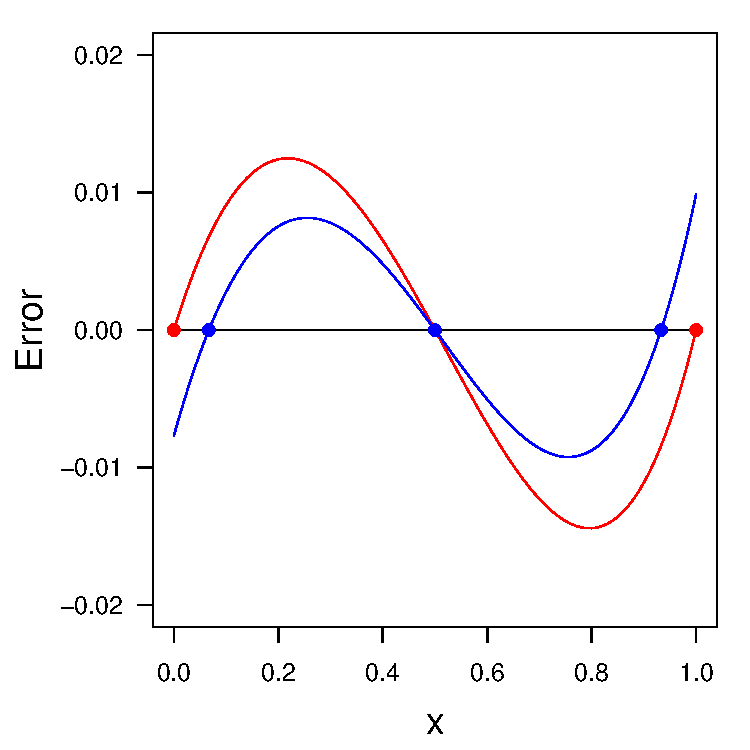
\includegraphics[width=\textwidth]{cheb_pts_lagr_err.pdf}

\end{minipage}
\caption{Lagrange interpolation of \(f(x) = e^x\) on \([0,1]\), but with Chebyshev points instead of equispaced points.}\label{fig::cheb_pts}
\end{figure}
%
Notice, from Figure~\ref{fig::cheb_zeros}, that the zeros accumulate or cluster near the boundary of the interval.  This helps to `clamp down' the polynomial interpolation near the boundary.
%
\begin{figure}[h!]\centering

\begin{minipage}[c]{0.48\textwidth}
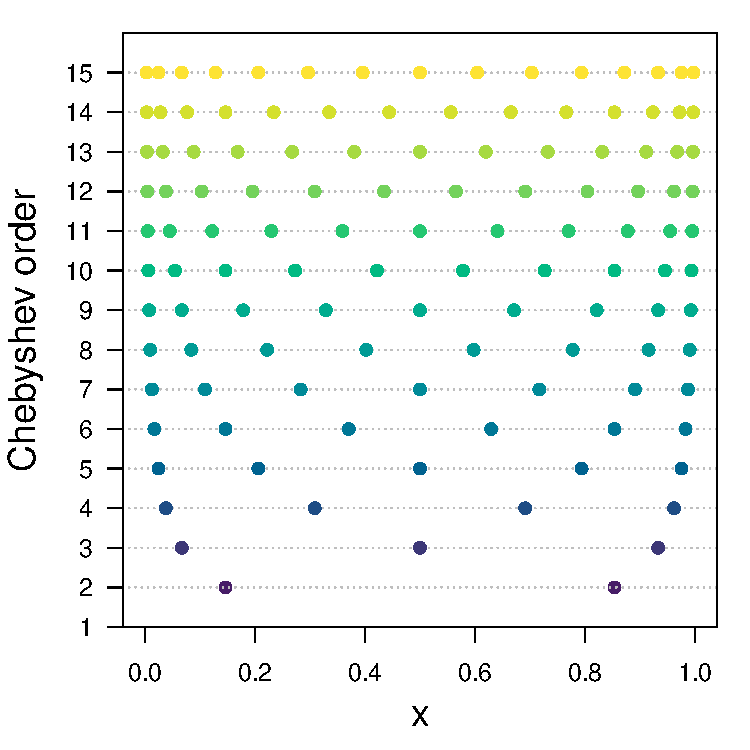
\includegraphics[width=\textwidth]{cheb_zeros.pdf}

\end{minipage}
\begin{minipage}[c]{0.48\textwidth}

\caption{Location of zeros to \(T_n(x)\) in the interval \([0, 1]\) for Chebyshev functions of orders from \(n=2, 3, \dots, 15\).}\label{fig::cheb_zeros}

\end{minipage}
\end{figure}


%%%%%%%%%%%%%%%%%%%%%%%%%%
%%%%%%%%%%%%%%%%%%%%%%%%%%
\subsubsection{Chebyshev economization}
As we will soon see, the `best' reduced order polynomial approximation \(P_{n-1}\) to a polynomial \(P_n(x)\) is given by \[P_{n-1}(x) = P_{n}(x) - a_n\tilde T_n(x)\] where \(\tilde T_n(x)\) is the \(n^\text{th}\) order monic Chebyshev polynomial and \(a_n\) is the coefficient of the highest order term in \(P_n(x)\).  To economize the polynomial approximation to \(f(x) = e^x\) given by a \(4^\text{th}\) order Maclaurin polynomial, we can subtract \(\dfrac{1}{24}\tilde T_4(x)\) from the original \(P_4(x)\) (note that \(a_4=\dfrac{1}{24}\) in the original polynomial representation).  This alters coefficients of all powers of \(x\)  of lower orders that are present in \(T_4(x)\) and eliminates the \(4^\text{th}\) order term entirely. Notice in Figure~\ref{fig::cheb_ord} that the maximum error for the third order function is only slightly worse for \(x=1.0\) than for the fourth order function.

\begin{figure}[h!]\centering
\begin{minipage}{0.48\textwidth}
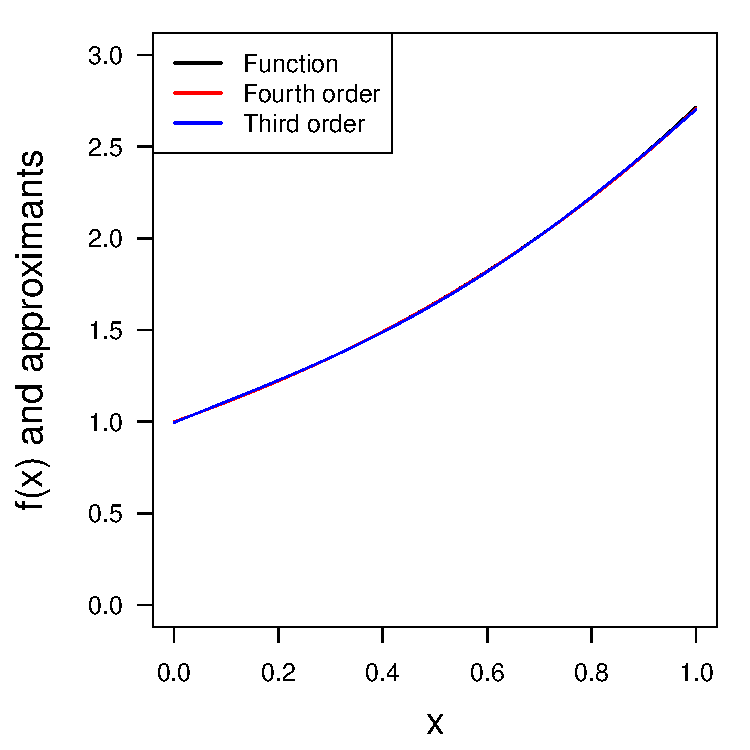
\includegraphics[width=\textwidth]{cheb_order_lagr.pdf}

\end{minipage}
\begin{minipage}{0.48\textwidth}

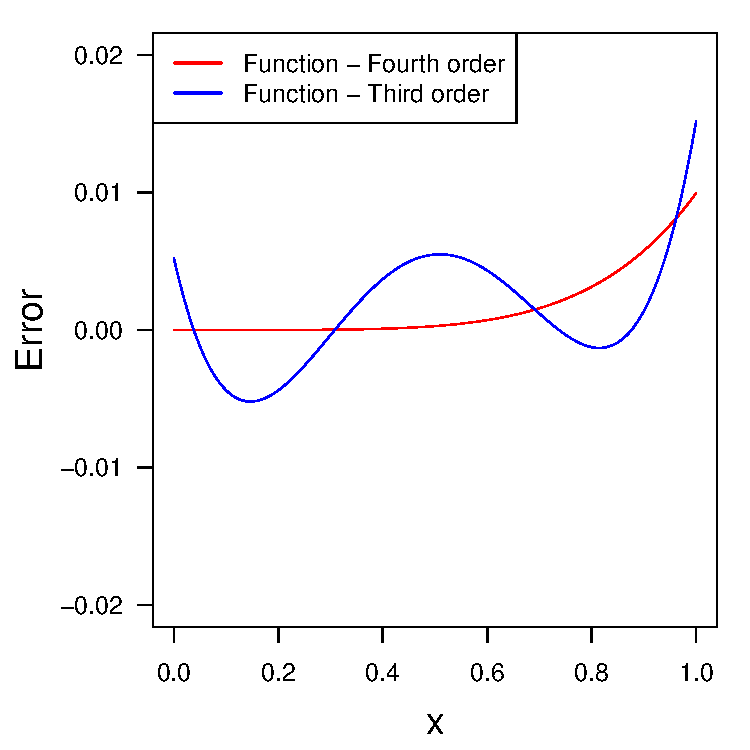
\includegraphics[width=\textwidth]{cheb_order_lagr_err.pdf}
\end{minipage}
\caption{Left: Full- and reduced-order approximations of \(f(x) = e^x\) on \([0, 1]\) by \(P_3(x)~=~P_4(x)~-~a_4 \tilde T_4(x)\). Right: Error in approximations of \(f(x) = e^x\) by full- and reduced-order polynomials.}\label{fig::cheb_ord}
\end{figure}

\end{document}